\documentclass[12pt]{article}

\oddsidemargin=.05in
\evensidemargin=.05in
\topmargin=-0.5in
\textwidth=6.5in
\textheight=9in
%\pagestyle{empty}

\usepackage{multicol}
\usepackage{amsmath,amssymb,amsthm}
\usepackage{easylist}
\usepackage{graphicx}
\newtheorem*{theorem}{Theorem}
\newtheorem*{claim}{Claim}
\newtheorem*{proposition}{Proposition}
\renewcommand{\qedsymbol}{\ensuremath{\blacksquare}}
\usepackage{fancyhdr}
\pagestyle{fancy}
\fancyhf{}
\lhead{Math 480 Project}
%\chead{Captain Scheduling for Ride the Ducks}
\rhead{Bickel and Yoon}
\cfoot{\thepage}

\usepackage{titlesec}

\titleformat{\section}
  {\normalfont\fontsize{15}{15}\bfseries}{\thesection}{1em}{}
\titleformat{\subsection}
  {\normalfont\fontsize{12}{15}\bfseries}{\thesection}{1em}{}

\begin{document}

\title{Captain Scheduling for Ride the Ducks of Seattle} 

\author{Zach Bickel and Michael Yoon}
\date{March 18, 2015}
\maketitle

\begin{abstract}
This paper describes the model and solution we derived from a scheduling problem for a 
small business, Ride the Ducks of Seattle. The objective was to create scheduling 
software that not only created a schedule, but also satisfied the wants and needs of the 
company as well as the workers. The problem is modeled as a Mixed Integer Problem 
and fitted with a branch and bound algorithm. After simplifying the problem at hand to 
fix the model we wanted to use, we were able to derive decision variables and a cost 
function to minimize. We used a two-step process. First, we began with a schedule 
creator with no branch and bound algorithm implemented simply to satisfy the constraints of the 
workers and the company. We then implemented the 
branch and bound algorithm to obtain a feasible solution with a better score than the original solution. Our finished product will be used 
by Ride the Ducks with the option of changing constraints to fit their week-to-week 
schedule making.
\end{abstract}


%\begin{multicols}{2}
\section*{Background}
Scheduling problems are very common for small businesses where many managers are still doing it by hand. Management at Ride the Ducks of Seattle currently spends upwards of ten hours per week scheduling captains for tours. Our goal is to build scheduling software that will drastically cut this time down and automatically build a schedule. This will be flexible enough so that a user will be able to update the constraints as they change. 

Ride the Ducks of Seattle offers continuous tours of downtown Seattle every day of the year except for Christmas, Christmas Eve and Thanksgiving. The Land \& Water Tour is a 90-minute tour that begins from two separate locations in downtown Seattle. Each tour is directed by a Captain, who operates an amphibious vehicle called a DUKW, also known as a duck. After each 90-minute tour is finished, there is a 30-minute break period for de-boarding the current tour, boarding the next tour, and a small break for the Captain. Each Captain will usually work 5 tours a day, 4 days a week, although there is a lot of variability from this in practice. Throughout this paper, we refer to 2-hour tour blocks, or simply 2-hour blocks, to denote a 90-minute tour followed by a 30-minute break period.

\begin{figure}[h!]
\centering
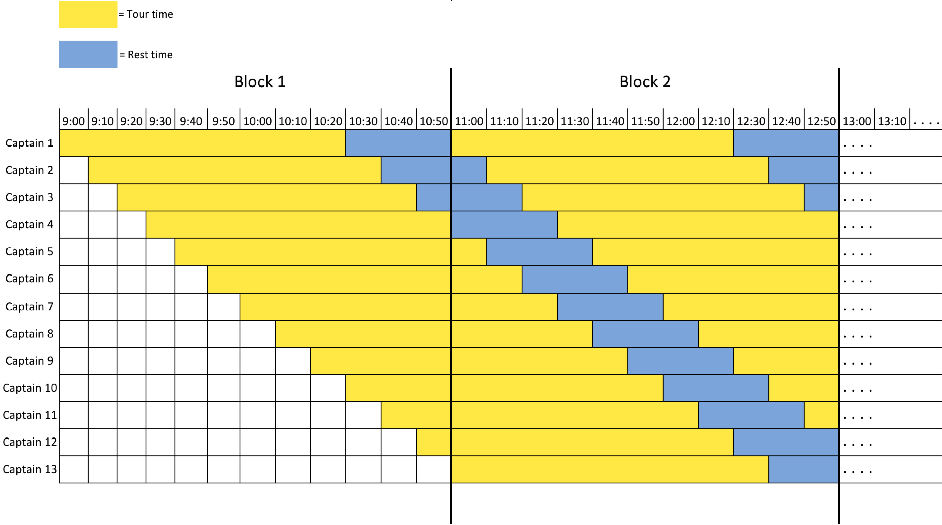
\includegraphics[scale=0.7]{block_figure2.png}
\caption{Staggered Block Structure}

\end{figure}

Scheduling the Captains in a way that satisfies the company as well as the 
individual Captains can be tricky. There are individual captain constraints that we have to deal with while filling the tours Ride the Ducks wants to run. Captain constraints can vary week to week and the amount of tours run in a day depends seasonally with the warmer seasons needing more tours than the cooler seasons. Due to the need of a flexible scheduling system, the notion of making the scheduling software easy to edit is crucial. The company can then 
make their own schedules with changing data. 

\section*{Goal}
Out goal is to automate a scheduling system for Ride the Ducks Captains to cover all shifts while satisfying each Captain's individual constraints. Note that we are simply attempting to find a feasible solution rather than an optimal solution since we do not have a clear objective function. % and attempting to minimize 4-day stretches.

\section*{Simplifications}
Ride the Ducks of Seattle is open 7 days a week from 9:00 AM to 9:00 PM at their main location and the same at their secondary location.  The company offers 90-minute tours where the driver ideally gets 30 minutes of rest before the next tour. There is one captain and one duck per tour. Each captain is not supposed to work more than four days a week and there are special constraints for individual captains, such as Captain A cannot work on Tuesday. Max 4 days worked for a Captain is a way to keep the workers rested and keep hours even among the captains that need them. We started by figuring out what a Ride the Ducks schedule looks like. The schedule is broken down into which captains are working what days and the times that day a Captain will be running a tour. The schedule also gives one or two captains that are on-call. From the schedule given by the company we were able to break down the schedule into main decisions. The decisions include, how many captains are available, how many captains we want in a day, how many time slots for tours, and a captains? restrictions on which days he or she can work. These decisions we believe are the most important to creating a schedule. The two different locations have been represented as one in our model. The two different locations run similarly such that we believe modeling one location is sufficient. The two locations are close to each other either. We also chose to run tours from 9:00 AM to 7:20 PM. With these decisions we made assumptions to certain aspects of the variables involved. For the tours, we capped the total length at 120 minutes which incudes the tour and rest time for the captains. The time slots for those tours are set to a default of one tour every 10 minutes. This allows for the most timeslots per 2-hour block these captains are working in. The number of captains in our problem is 40, with 18 captains scheduled a day. Currently the model does not include on-call workers, just creates a schedules where all captains assigned that day are working. We chose to extend the hours Ride the Ducks of Seattle are open so that they have more flexibility with tours and start times. With these model time hours, we were able to simplify the blocks of tours to 6 blocks of tours per day. Rather than count the number of hours the captains works per week, we have decided to keep track of the number of days a captain has worked. Due to our block structure, we are able to keep track of how many blocks worked in a day. The number of blocks is maxed out at 6 blocks for a 12-hour opening. So, if a Captain is to work 4 days a week running a tour at all 6 blocks a day it comes out to 48 hours. 48-hours being the max number of hours and days worked a Captain can work in our schedule.  These simplifications allow us to created our decision variables and constraints in a clear way so we can tackle our problem.

\section*{Literature Overview}
Before we tried to model the problem at hand, we read research papers on modeling problems similar to our own. One paper we came across discussed America West and the Arizona State University using a mathematical model to decide on an optimal airplane boarding strategy (Hogg, 2002). We gained more insight on handling mixed integer problems and how they are modeled. We were able to better derive the decision variables in our own problem after learning about how the ASU and America West team simplified their problem. The ASU and America West team simplified the problems of boarding an airplane by classifying the problems into two groups (Hogg). This helped us to understand how to simplify our own constraints as well as which decision variable we wanted to minimize. Simplifying the problem gave us more flexibility on how to represent Captains and the timeslots.

Patrick Perkins paper on creating weekly timetables for the Math Study Center at the University of Washington was another similar modeling problem (Perkins, 2004). Perkins? modeling problem was to generate optimal weekly timetables for tutors at the Math Study Center using similar constraints to our problem. Their team chose to model the scheduling problem as an Integer Programming problem as opposed to heuristics, which was how the schedules were first made (Perkins, 2004). Perkins? team tackled their scheduling problem in a two-step process. The first step of their modeling process utilized a relaxed version of constraints to obtain a workable schedule. This involved a ?constraint relaxation approach? where constraints are created to remove unwanted types of schedules immediately (Perkins, 2004). From the schedules left, Perkins? team utilizes their ?penalty approach? which tries to maximize their objective function to figure out the best possible schedule. Perkins states that these schedules are better optimized and thus produce more efficient schedules. We took this two-step process and modified Perkins? group approaches to better fit our model. We too wanted to model our scheduling problem using Integer Programming. Nicholas Beaumont and his team wrote a paper on scheduling staff that drove to and serviced customers (Beaumont, 1997). 

In Beaumonts case study, the staff he was trying to schedule had many similarities to the staff we were trying to schedule. This included constraints on the staff based on times they could work and the demand of their work (Beaumont, 1997). Using binary values and other variables assigned to certain staff members to restrict their start times was something that we wanted to implement in our model. These constraints changed by week for our own partner, thus fully understanding the formulation of these constraints was necessary to write up code that would create these constraints for our partner once we hand them our final product. Similar to this, the demand of the staff in Beaumonts study and our own problem of varying numbers of tours based on the time of year. These papers offered us guidance on our own problem and model. Simplify the process; solve the problem two-step approach and how to model certain restrictions that may change based on the situation. All of the ideas listed we utilized to give our partners the best possible solution. 
\section*{Variables and Parameters} First, let's define some parameters:
\begin{align*}
n &\equiv \text{Number of captains,}\\
m &\equiv \text{Number of tour slots per 2-hour block,}\\
b &\equiv \text{Number of 2-hour blocks in one day,}\\
k &\equiv \text{Number of time slots per day.}
\end{align*}
If there are $n$ captains and $k$ time slots in a day, then there are $7kn$ decision variables. Note that $k = mb$. Our decision variables will represent when the captains will run a tour. We can understand them as a matrix $X$, where $x_{ijd}$ = 1 if captain $i \in \{1, 2, \dots, n\}$ runs a tour at time $j \in \{1, 2, \dots k\}$ on day $d \in \{1, 2, \dots, 7\}$ and 0 otherwise.

%\section*{Objective Function}
%Our objective function will represent the number of 4-day stretches captains have to work and our goal will be to minimize this %in order to keep captain fatigue low. For readability purposes, let's define a separate function $w(i, d)$ to represent captain %$i$ working on day $d$:
%$$w(i,d) = \sum_{j = 1}^{k}{x_{ijd}}.$$
%So, $w(i,d) = 1$ if captain $i$ works on day $d$ and 0 otherwise. Then $w(i, 1)w(i, 2)w(i, 3)w(i, 4) = 1$ implies that captain %works on days 1, 2, 3 and 4. Our objective function $f$ is thus:
%$$f(i) = [w(i, 1) \cdots w(i, 4)] + [w(i, 2) \cdots w(i, 5)] + \cdots + [w(i, 4) \cdots w(i, 7)] + [w(i, 5) w(i, 6) w(i, 7) %w(i,1)].$$
%Note that the last term in the function wraps around to make sure that we are not loading the schedule too heavily towards the %weekend shifts.

\section*{Constraints}
First, we have to define 
$w_{id}$ to be 1 if Captain $i$ works on day $d$ an 0 otherwise. So, for Captain $i$ on day $d$, 

$$w_{id} = \begin{cases} 1 & \mbox{if } \sum_{j = 1}^{k}x_{ijd} \ge 1,\\
0 & \mbox{otherwise}. \end{cases}$$

\begin{enumerate}
\item[(1)] Captain requested tour constraint: Ride the Ducks offers special tours for large groups (birthdays, corporate events,  etc.). Some captains are requested to run these specific tours by the group, so if captain $i$ is requested on
day $d$ at time slot $j$,
$$x_{ijd} = 1.$$
\item[(2)] Time between tours constraint: A Captain needs 2-hours between each of their tours in a given day. 
For each pair of tour slots, $j$ and $j'$, run by Captain $i$ on day $d$, such that $j \neq j'$,
$$\lvert j - j'\rvert \ge m.$$
Ideally, this would be an equality constraint, but constraint (6) may make this impossible if a Captain is requested to run several tours that are on different block cycles. 
\item[(3)] Number of days worked per week constraint: For the most part, each captain can work a maximum of 4 days per week although it can vary. We'll define the maximum number of days captain $i$ can work as $y_i$.
For each captain $i$,
$$\sum_{d = 1}^{7}w_{id}\le y_i.$$
\item[(4)] Captain unavailability constraint: If captain $i$ is unavailable on day $d$,
$$\sum_{j = 1}^{k}{x_{ijd}} = 0.$$
\item[(5)] Tours per time slot constraint: We would like to have a certain number of tours staring at each time slot. If we want $t_{jd}$ tours at time slot $j$ on day $d$,
$$\sum_{i = 1}^{n}{x_{ijd}} = t_{jd}.$$
\item[(6)] Number of daily captains constraint: We want to have $c_d$ captains at work on day $d$. This means that, for day $d$, 
$$\sum_{i = 1}^{n}{w_{id}} = c_d.$$
\end{enumerate}
Constraints (1) through (4) are individual Captain constraints while constraints (5) and (6) are company constraints. 

\section*{Algorithm and Commentary}
The algorithm we used to obtain a solution is similar to the one used in Perkins, 2004 to obtain a feasible solution. It involves assigning tours in the fashion of a greedy algorithm, paying attention to Captain constraints (1) -(4), with the goal fulfilling constraints (5) and (6). Since we utilize a greedy algorithm, constraints (5) and (6) may not be met with one pass, so we implemented an approach that would use multiple passes and relax constraints as needed to get a feasible solution. 

\subsection*{Algorithm}
\begin{itemize}
\item[(1)] If a Captain has requested tours, assign them their requested tour(s). For each day where a Captain has requested tours, fill in the Captain’s schedule for that day so that they work other tours that Ride the Ducks wishes to run. We schedule around the requested tours so that the Captains have a full five tours in the days that they are requested.

\item[(2)] Loop through every Captain on each day for each tour time slot. If the Captain did not work the day before or after, no individual constraints are violated, and a tour is unfilled at that particular time slot on that day, assign the Captain to the particular tour.

\item[(3)] If some tours have not been filled, attempt to fill in all open tours with Captains whose individual constraints would not be violated by assigning them to unfilled tours.

\item[(4)] If there are still unfilled tours, relax individual constraints  (first (3), then (4) if it still fails) and give a report to management so they can choose captains that may be able to cover unfilled tours.

\end{itemize}

\subsection*{Commentary}
\begin{itemize}

\item[(1)] Note that the requested tours may occur off-cycle. For example, a Captain has requested tours at 9:20 in the morning and 12:00 in the afternoon. In this case, the Captain will need a longer break in order to get onto a new cycle (runs 9:20 and 12:00 rather than 9:20 and 11:20). 

\item[(2)] Note that this fills Captains into tours so that they don't have to work two days in a row in a given week. This step essentially breaks the captains into two groups and has each group run on alternate days. Because of the nature of the captain constraints, we will not be able to fully break the captains into alternating groups and fully satisfy constraints (5) and (6), so we'll have to go through the captains again without the alternating scheme to fill in more tours.

\item[(3)] In this step, we are filling in what the alternating scheme could not fill in from part (2). If a feasible schedule exists, it will be found in this step.

\item[(4)] In this step, we are dealing with an infeasible schedule. Some captains have softer constraints that can be relaxed in special circumstances (i.e. can actually work 5 days) that are hard to put into software. We want to run these relaxations by management and the captains before making a decision. 

\end{itemize}

\section*{Results} 

\begin{figure}[h!]
\centering
\includegraphics[scale=1]{"Example_Schedule".png}
\caption{Example of Captain Schedule.}
\end{figure}
The schedules being created by our code are feasible. They stay within the constraints for all schedules as well as complying with individual constraints set by captains themselves. Our first schedules were more automated and did not include any of the individual captains constraints. The schedules satisfied the number of tours and captains per day, tours per timeslot, and number of days worked. The captains were being assigned in two groups that alternated. This allowed for a feasible schedule based on most of Ride the Ducks’ constraints. This also allowed for captains to be rested between days they worked. Of course, these schedules are not ideal since they do not satisfy all of the individual constraints. We then added the individual constraints. (references figure) we see a one schedule created by our code. It includes (here, put the constraints in). This schedule satisfies more of the individual constraints while satisfying most of company’s constraints. We believe that Ride the Ducks will still be able to use the schedules created to their advantage. Putting more emphasis on the individual constraints of captains means when finishing the schedule, we have allowed Ride the Ducks to focus more on filling their tours with captains rather than dealing with such specific constraints that seem to slow the schedule making process the most. Dealing less with the detailed constraints and more on constraints that can be more easily handled thus lowering the total amount of time needed to complete a schedule for Ride the Ducks. The code itself runs quickly. The code will generate a schedule under a minute. The time it takes to create the constraints for the code is also quite fast. We believe assigning each individual constraint by hand is a small price to pay in the overall creation of a schedule. The number of tours and captains are also inputted by hand and are simple to update. The schedules are saved to a Comma Separated Values (CSV) that the user can readily open, edit, and print. 


\section*{Improvements}
There are several improvements that can be made. First of all, our algorithm only finds a feasible solution to the scheduling problem. Another step could be added to use an objective function to score different feasible schedules and use a branch and bound algorithm to find a schedule with a better score than the initial feasible solution. Potential objective functions might be along the lines of assigning a value to the balance of a schedule or assigning a measure of fairness. Other improvements could be made regarding how users interface with the software. Currently, constraints are kept in CSV files but they could be transferred into a more intuitive format with a GUI. Other improvements could involve relaxing some of the simplifications by treating separate locations differently and adding in the two extra backup captains. 

\section*{Conclusion}

\section*{Acknowledgments}
Barack Obama, Mike Jones. 

%\end{multicols}

\begin{thebibliography}{9}
\bibitem{beaumont}
Beaumont, Nicholas. \emph{Scheduling staff using mixed integer programming.} European journal of operational research 98.3 (1997): 473-484.

\bibitem{airline}  
 Van Den Briel, Menkes HL, et al. \emph{America west airlines develops efficient boarding strategies.} Interfaces 35.3 (2005): 191-201.

\bibitem{perkins}
White, Caleb Z., et al. \emph{Creating weekly timetables to maximize employee preferences.} The UMAP J 25 (2004): 5-25.


\end{thebibliography}

\end{document}